%%%%%%%%%%%%%%%%%%%%%%%%%%%%%%%%%%%%%%%%%
% Beamer Presentation
% LaTeX Template
% Version 1.0 (10/11/12)
%
% This template has been downloaded from:
% http://www.LaTeXTemplates.com
%
% License:
% CC BY-NC-SA 3.0 (http://creativecommons.org/licenses/by-nc-sa/3.0/)
%
%%%%%%%%%%%%%%%%%%%%%%%%%%%%%%%%%%%%%%%%%

%----------------------------------------------------------------------------------------
%	PACKAGES AND THEMES
%----------------------------------------------------------------------------------------

\documentclass{beamer}

\mode<presentation> {

% The Beamer class comes with a number of default slide themes
% which change the colors and layouts of slides. Below this is a list
% of all the themes, uncomment each in turn to see what they look like.

%\usetheme{default}
%\usetheme{AnnArbor}
%\usetheme{Antibes}
%\usetheme{Bergen}
%\usetheme{Berkeley}
%\usetheme{Berlin}
%\usetheme{Boadilla}
%\usetheme{CambridgeUS}
%\usetheme{Copenhagen}
\usetheme{Darmstadt}
%\usetheme{Dresden}
%\usetheme{Frankfurt}
%\usetheme{Goettingen}
%\usetheme{Hannover}
%\usetheme{Ilmenau}
%\usetheme{JuanLesPins}
%\usetheme{Luebeck}
%\usetheme{Madrid}
%\usetheme{Malmoe}
%\usetheme{Marburg}
%\usetheme{Montpellier}
%\usetheme{PaloAlto}
%\usetheme{Pittsburgh}
%\usetheme{Rochester}
%\usetheme{Singapore}
%\usetheme{Szeged}
%\usetheme{Warsaw}

% As well as themes, the Beamer class has a number of color themes
% for any slide theme. Uncomment each of these in turn to see how it
% changes the colors of your current slide theme.

%\usecolortheme{albatross}
%\usecolortheme{beaver}
%\usecolortheme{beetle}
%\usecolortheme{crane}
%\usecolortheme{dolphin}
%\usecolortheme{dove}
%\usecolortheme{fly}
%\usecolortheme{lily}
%\usecolortheme{orchid}
%\usecolortheme{rose}
%\usecolortheme{seagull}
%\usecolortheme{seahorse}
%\usecolortheme{whale}
%\usecolortheme{wolverine}

%\setbeamertemplate{footline} % To remove the footer line in all slides uncomment this line
\setbeamertemplate{footline}[frame number] % To replace the footer line in all slides with a simple slide count uncomment this line

%\setbeamertemplate{navigation symbols}{} % To remove the navigation symbols from the bottom of all slides uncomment this line
}

\usepackage{graphicx} % Allows including images
\usepackage{booktabs} % Allows the use of \toprule, \midrule and \bottomrule in tables
\usepackage[T1]{fontenc}
\usepackage{tikz}
%\usepackage{svg}
%\usepackage[useregional]{datetime2}
\newcommand{\maybe}[1]{\textcolor{gray}{#1}}

%\begin{filecontents}{\jobname.bib}
%@article{cohan2018smhd,
  %title={SMHD: A Large-Scale Resource for Exploring Online Language Usage for Multiple Mental Health Conditions},
  %author={Cohan, Arman and Desmet, Bart and Yates, Andrew and Soldaini, Luca and MacAvaney, Sean and Goharian, Nazli},
  %journal={arXiv preprint arXiv:1806.05258},
  %year={2018}
%}
%\end{filecontents}
%\usepackage[style=authoryear]{biblatex}
%\renewcommand*{\nameyeardelim}{\addcomma\addspace}

%\addbibresource{prez.bbl}

%\usepackage[backend=biber,
%style=alphabetic,
%citestyle=authoryear]
%{biblatex}
%\addbibresource{prez.bib}
%\usepackage[round]{natbib}
 
%----------------------------------------------------------------------------------------
%	TITLE PAGE
%----------------------------------------------------------------------------------------

\title[Bipolar Disorder Prediction]{Not Just Depressed:\\Bipolar Disorder Prediction on Reddit} % The short title appears at the bottom of every slide, the full title is only on the title page

\author{Ivan Sekuli\'c, Matej Gjurkovi\'c, Jan \v{S}najder} % Your name
\institute[University of Zagreb] % Your institution as it will appear on the bottom of every slide, may be shorthand to save space
{
Text Analysis and Knowledge Engineering Lab \\
University of Zagreb \\ % Your institution for the title page

\includegraphics[scale=0.2]{imgs/TakeLab-LOGO-default.pdf}
%\medskip
%\textit{our.emails@wat.com} % Your email address
}
%\date{\today} % Date, can be changed to a custom date
\date{WASSA\,@\,EMNLP, Brussels\\31 October, 2018}

\setbeamertemplate{navigation symbols}{}

\begin{document}
%\bibliographystyle{plainnat}
%\bibliography{prez}

\begin{frame}
\titlepage % Print the title page as the first slide
\end{frame}

\begin{frame}
  \frametitle{Motivation}
  \centering
  How does everyday language reflect basic social and personality processes?
\end{frame}

\begin{frame}
  \frametitle{Motivation}
  \centering
  How does everyday language reflect our mental health?
\end{frame}

\begin{frame}
  \frametitle{Motivation}
  \centering
  Can text and emotion analysis help with bipolar disorder detection?
\end{frame}

\begin{frame}
\frametitle{Overview} % Table of contents slide, comment this block out to remove it
\tableofcontents % Throughout your presentation, if you choose to use \section{} and \subsection{} commands, these will automatically be printed on this slide as an overview of your presentation
\end{frame}

%----------------------------------------------------------------------------------------
%	PRESENTATION SLIDES
%----------------------------------------------------------------------------------------

%------------------------------------------------
\section{Introduction} % Sections can be created in order to organize your presentation into discrete blocks, all sections and subsections are automatically printed in the table of contents as an overview of the talk
%------------------------------------------------

\begin{frame}
\frametitle{Mental health \& language}
\textbf{The Mental Health issue}
\begin{itemize}
  \item Up to 27\% of Europe population suffer or have suffered from some kind of mental disorder \maybe{(WHO, 2017; Wykes et al., 2015)}
  \item 35--50\% go undiagnosed
\end{itemize}



\textbf{Language analysis} for \textbf{deeper understanding} and \textbf{early detection} of illnesses:
\begin{itemize}
  \item Depression \maybe{(Rude et al., 2004; De Choudhury et al., 2013)}, anxiety \maybe{(Shen and Rudzicz, 2017)}, PTSD \maybe{(Coppersmith et al., 2015)}, schizophrenia \maybe{(Benton et al., 2017)}, bipolar disorder \maybe{(Kramer et al., 2004)}
\end{itemize}
\end{frame}

%------------------------------------------------

\begin{frame}
\frametitle{Bipolar Disorder}
%Psychiatric disorder characterized by: \maybe{an image of a graph going up and down?}
\begin{itemize}
  \item Uncontrolled changes in mood and energy levels
  \item Manic and depressive episodes 
  \item Recurrent phases that differ in intensity and duration

\end{itemize}

%\begin{tikzpicture}
%\draw (0,0) .. controls (0,2) and (4,0) .. (4,2);
%\end{tikzpicture}

\begin{center}
%\includegraphics[scale=0.18]{bipolar-img1.jpg}
\includegraphics[width=8cm,height=2.5cm]{imgs/bipolar-img1.jpg}
\end{center}


Why is research on bipolar disorder important?
\begin{itemize}
  \item Affects more than 60M people worldwide %\maybe{(Anderson et al., 2012)}
  \item High suicide rate (more than 6\%) %\maybe{(Nordentoft et al., 2011)}
\end{itemize}
\end{frame}

%------------------------------------------------

\section{Dataset}
\begin{frame}
\frametitle{Reddit: a gold mine for user-generated text}
\begin{columns}
  \column{0.80\linewidth}
    \textbf{Reddit}
  \begin{itemize}
    \item One of the largest social media sites in the world
    \item User anonymity
    \item Wide range of topics
\end{itemize}

%\includesvg{logo}
  \column{0.2\linewidth}
    
\includegraphics[scale=0.06]{imgs/redditlogo.png}
\end{columns}

\vspace{4 mm}

\begin{columns}
  \column{1\linewidth}
\textbf{Self-reported mental disorders}
\begin{itemize}
  \item Bipolar-related subreddits: \textit{bipolar, bipolar2, BipolarReddit, BipolarSOs, bipolarart}
  \item Search for \textit{``I am diagnosed with bipolar''} in user's comments
  \item Inspect users' \textit{flairs} \maybe{(following Gjurkovi\'c and \v{S}najder, 2018)}: \textit{``Bipolar''}, \textit{``BP1''}, etc.
\end{itemize}
\column{0.0\linewidth}

\end{columns}
\end{frame}

\begin{frame}
  \frametitle{Self-reported Bipolar Disorder}
\begin{center}
%\includegraphics[scale=0.2]{../Pictures/diagnoseddd4.png}
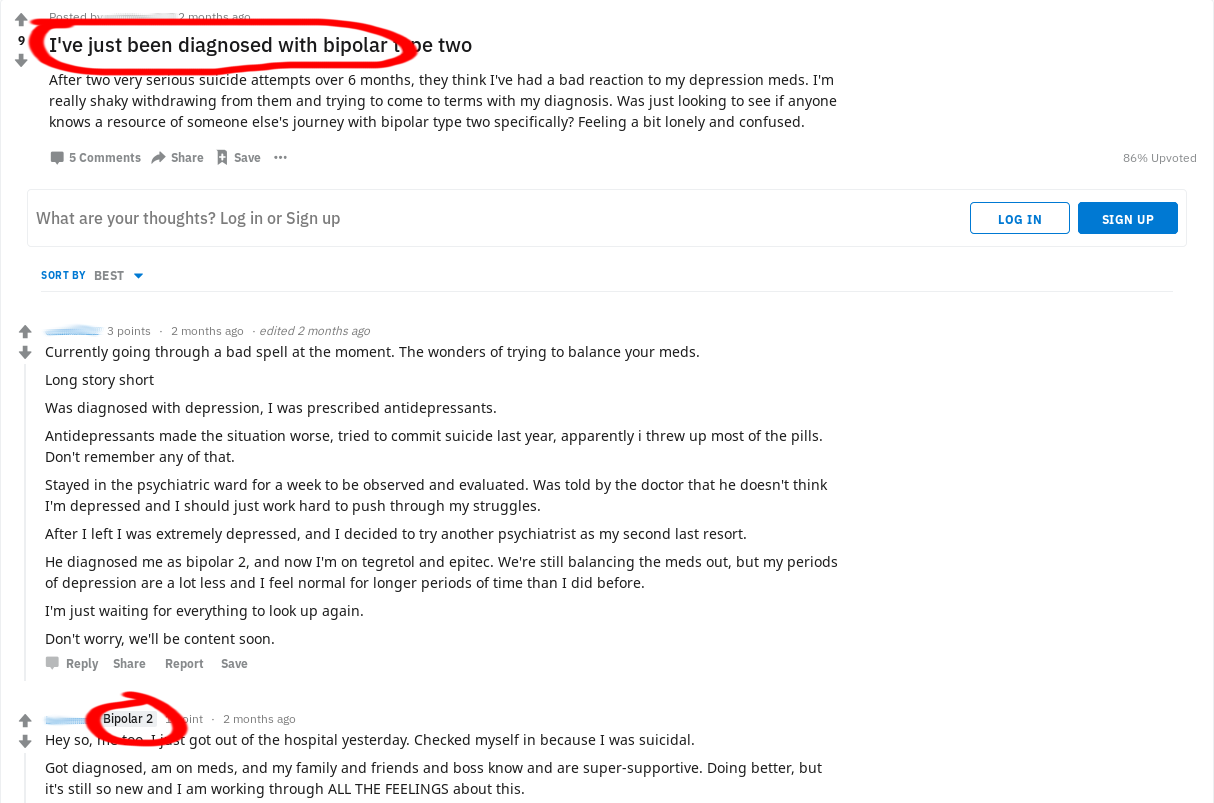
\includegraphics[scale=0.2]{imgs/edited2.png}
\end{center}

\pause
\begin{itemize}
  \item Compiled a \textbf{control group} to represent general Reddit population
\end{itemize}

\end{frame}



\begin{frame}
  \frametitle{Dataset pruning}

  Cleaning the dataset:
  \begin{itemize}
    \item Removed all comments on bipolar-related subreddits, as well as on the general \textit{mentalhealth} subreddit
    \item Removed all comments that had \textit{``bipolar''} or \textit{``BP''} in them
    \item Keep only users with > 1000 words left resulting in \textbf{{\raise.17ex\hbox{$\scriptstyle\sim$}}3.5k bipolar users}
  \end{itemize}


\pause
Parallel work by Cohan et al. (2018): gathered 36k users labeled with 9 mental disorders


\end{frame}
\begin{frame}
  \frametitle{Topical Categories}
  \begin{itemize}
    \item Additional topic \textbf{bias reduction}
    \item Manually grouped top {\raise.17ex\hbox{$\scriptstyle\sim$}}400 subreddits in the categories below:
  \end{itemize}
\begin{table}
\centering
{\small
\begin{tabular}{lrr}
\toprule
Category            & \#~bipolar   & \#~control   \\
\midrule
Animals               & 397  & 898  \\
AskReddit             & 1797 & 2767 \\
Gaming                & 489  & 1501 \\
Jobs and finance      & 293  & 586  \\
Movies/music/books    & 502  & 1606 \\
Politics              & 332  & 2445 \\
Religion              & 264  & 700  \\
Sex and relationships & 948  & 1000 \\
Sports                & 156  & 785 \\
\midrule
All                   & 3488 & 3931 \\
\bottomrule
\end{tabular}}
%\caption{\label{tbl:categories} The number of unique bipolar disorder and control group users broken down by topic categories}
\end{table}
\end{frame}


\section{Bipolar Disorder Prediction}
\begin{frame}
  \frametitle{Feature Extraction}
  (1) Psycholinguistic features:
\begin{itemize}
  \item \textbf{LIWC} \maybe{(Pennebaker et al., 2015)} -- classify the words into dictionary-defined categories (syntactic, topical, psychological features)
  \item \textbf{Empath} \maybe{(Fast et al., 2016)} -- based on neural embeddings (200 manually curated categories)
\end{itemize}
(2) Lexical features -- tf-idf weighted bag-of-words

(3) Reddit user features -- post/comment ratio, \#\textit{gilded} posts, \textit{ups}--\textit{downs}, time intervals between comments
\end{frame}

\begin{frame}
  \frametitle{Results}
  \begin{itemize}
    \item Binary classification task
    \item Models: SVM, Logistic Regression, Random Forest
    \item 10x5 nested cross-validation
  \end{itemize}

  %\maybe{-show the table with features and classifiers? if so, remove the first one}
\begin{table}[t]
\centering
{\small
\begin{tabular}{lrr}
\toprule
\multicolumn{1}{l}{} & \multicolumn{1}{c}{Acc} & \multicolumn{1}{c}{F1} \\
\midrule
MCC                   & 0.529                       &  --                     \\
Random                & 0.546                       & 0.453                  \\
SVM                   & 0.865                       & 0.853                  \\
%LinSVM                & 0.864                       & 0.852                  \\
LogReg                & 0.866                       & 0.849                  \\
RF                    & \textbf{0.869}              & \textbf{0.863}        \\
\bottomrule
\end{tabular}}
%\caption{\label{tbl:rez_all} Prediction accuracy and F1-scores}
\end{table}

\end{frame}

\begin{frame}
  \frametitle{Per-category results}
  * two-sided t-test, p$<$0.001
\begin{table}[t]
\centering
{\small
\begin{tabular}{lrr}
\toprule
                      & MCC   & Our models \\
\midrule
Animals               & 0.693 & 0.807*      \\
AskReddit             & 0.606  & 0.856*      \\
Gaming                & 0.754  & 0.777*     \\
Jobs and finance      & 0.665 & 0.752*      \\
Movies/music/books    & 0.761 & 0.817*      \\
Politics              & 0.880  & 0.882*      \\
Religion              & 0.724  & 0.784*      \\
Sex and relationships & 0.513 & 0.801*      \\
Sports                & 0.832  & 0.837\phantom{*}     \\
\bottomrule
\end{tabular}}
%\caption{\label{tbl:rez_cat} Accuracy of the MCC baseline and our models across topic categories.
%Accuracies marked with ``*'' are significantly different from the baseline.}
\end{table}
\end{frame}

\section{Feature Analysis}
\begin{frame}
  \frametitle{Feature Analysis}
  %\maybe{Two-sided t-test, with the null hypothesis of no difference in feature values between users
  %with bipolar disorder and control users, p$<$0.001}

\begin{table}[]
\centering
{\small
\begin{tabular}{lrr}
\toprule
Feature    & Bipolar $\mu$    & Control $\mu$    \\ 
\midrule
  pronoun    & \textbf{16.87} & 14.86 \\
  ppron             & \textbf{10.69} & 8.66  \\
  i                & \textbf{5.84}  & 3.38  \\
  article     & 5.88  & \textbf{6.55} \\
  health           & \textbf{0.96}  & 0.50  \\
  feel       & \textbf{0.69}  & 0.48  \\
  power     & 2.11  & \textbf{2.58}  \\
  bio         & \textbf{2.65}  & 1.90  \\
  Authentic        & \textbf{52.65} & 32.92 \\
  Clout       & 48.51 & \textbf{58.03} \\
%conj   & 6.70 &  6.04 \\
%Analytic  & 41.27 & 50.82 \\
%they   &  0.88 &   1.11 \\
%anger   &  0.81 &  1.12 \\
%time   & 4.60 &  4.06 \\
%Tone & 52.16 & 41.92 \\    % maybe interesting? Emotional tone
%posemo & 3.89 &   3.44 \\
%sad & 0.45 &  0.36 \\
\bottomrule
\end{tabular}}
%\caption{\label{tbl:liwc} Mean values of most significant LIWC features for both groups}
\end{table}
In line with previous research on depression: Personal pronoun \textit{I} \maybe{(Stirman and Pennebaker, 2001; Rude et al., 2004)}%\maybe{(cite and go into details?)}
\end{frame}

\begin{frame}
  \frametitle{Per-category analysis}
  %Remove the slide -> no time
\begin{table}[]
\begin{tabular}{lccccccc}
  \toprule
Feature   & Authentic & i & health & feel & power & bio & article \\
\midrule
Animals&+&+&+&+&+&+&+\\
AskReddit&+&+&+&+&+&+&+\\
Gaming&+&+&&&&&+\\
Jobs&+&+&+&+&+&+&+\\
Movies&+&+&+&+&+&+&+\\
Politics&+&+&+&+&&+&+\\
Religion&+&+&+&+&+&&+\\
Sex&+&+&+&+&+&+&+\\
Sports&+&+&&+&&&
\bottomrule
\end{tabular}
\end{table}

+ signals significant difference in feature value between bipolar and control group

%\begin{table}[]
%\begin{tabular}{lccccccccc}
%Feature   & \multicolumn{1}{l}{Animals} & \multicolumn{1}{l}{AskReddit} & \multicolumn{1}{l}{Gaming} & \multicolumn{1}{l}{Jobs} & \multicolumn{1}{l}{Movies} & \multicolumn{1}{l}{Politics} & \multicolumn{1}{l}{Religion} & \multicolumn{1}{l}{Sex} & \multicolumn{1}{l}{Sports} \\
%Authentic&+&+&+&+&+&+&+&+&+\\
%ppron&+&+&+&+&+&+&+&+&+\\
%i&+&+&+&+&+&+&+&+&+\\
%health&+&+&&+&+&+&+&+&\\
%feel&+&+&&+&+&+&+&+&+\\
%power&+&+&&+&+&&+&+&\\
%pronoun&+&+&+&+&+&+&+&+&\\
%bio&+&+&&+&+&+&&+&\\
%Clout&+&+&+&+&+&+&+&+&+\\
%article&+&+&+&+&+&+&+&+&
%\end{tabular}
%\end{table}
  %\maybe{- say which categories yield the same results, and which differ a bit}

    %\maybe{Maybe a table [Top 10 features] x [Categories] --> '+' where the feature is significant}
\end{frame}

\section{Emotion Analysis}
\begin{frame}
  \frametitle{Emotion-expressive words analysis}
  %- Between-group differences
  LIWC emotion-related categories
\begin{table}
\centering
{\small
\begin{tabular}{lrr}
\toprule
Feature & Bipolar $\mu$  & Control $\mu$ \\
\midrule
  affect & \textbf{6.415} & 6.074 \\
  posemo & \textbf{3.899} & 3.442 \\
  negemo & 2.432 & \textbf{2.569} \\
  anxiety & \textbf{0.367} & 0.266 \\
  anger & 0.818 & \textbf{1.128} \\
  sad & \textbf{0.455} & 0.363 \\
\bottomrule
\end{tabular}}
%\caption{\label{tbl:emoemo} Means and standard deviations of LIWC emotion categories for bipolar and control group} 
\end{table}
  
\end{frame}

\begin{frame}
  \frametitle{User-level emotion variance}
  \begin{itemize}
    \item Split comments of 100 users (of both groups) with more than 100K words into \textbf{monthly chunks}
    \item Calculate LIWC features for each month and compute their \textbf{standard deviations}
  \end{itemize}

  \pause

\begin{table}
\centering
{\small
\begin{tabular}{lrrr}
\toprule
        & Bipolar       & Control  & p-value     \\
\midrule
posemo  & 0.00272* & 0.00166 & 0.00272\\
negemo  & 0.00583*  & 0.00379 & 0.00583\\
anxiety & 0.00765* & 0.00627 & 0.00765\\
anger   & 0.01745\phantom{*}  & 0.01422 & 0.01745 \\
sadness & 0.00695* & 0.00572 & 0.00695\\
\bottomrule
\end{tabular}}
%\caption{\label{tbl:emo} Averages of standard deviations in the use of emotion-expressive words for the two groups. All differences are significant except for ``anger''.} 
\end{table}
\centering
* p$<$0.01; averages of SDs in the use of emotion-expressive words

\end{frame}

\begin{frame}
  \frametitle{Wrapping up}
  \textbf{Conclusion}
  \begin{itemize}
    \item preliminary study of bipolar disorder 
    \item benchmark classification results (86\% accuracy)
    \item psycholinguistic and emotion-related feature analysis
  \end{itemize}

  \textbf{Future work}
  \begin{itemize}
    \item Detect manic and depressive episodes -- compare to clinical depression%Compare to the clinical depression
    \item Deep learning for prediction
  \end{itemize}
\end{frame}

%------------------------------------------------


\begin{frame}
  \frametitle{Not Just Depressed: Bipolar Disorder Prediction on Reddit}

  \centering
  Ivan Sekuli\'c, Matej Gjurkovi\'c, Jan \v{S}najder

  \vspace{4 mm} 

  \textbf{ivan.sekulic@h-its.org}

  \textbf{takelab@fer.hr}


\Huge{\centerline{Thank you!}}
\end{frame}

\begin{frame}[noframenumbering]
  \frametitle{LIWC vs Empath vs tf-idf}
\begin{table}[t]
\centering
{\small
\begin{tabular}{lrrrr}
\toprule
       & LIWC  & Empath & Tf-idf & All   \\ 
\midrule
SVM    & 0.837 & 0.782  & \textbf{0.865}  & 0.838 \\
%LinSVM & 0.833 & 0.818  & \textbf{0.864}  & 0.835 \\
LogReg & 0.841 & 0.819  & \textbf{0.866}  & 0.862 \\
RF     & 0.829 & 0.825  & 0.869  & \textbf{0.869} \\
\bottomrule
\end{tabular}}
%\caption{\label{tbl:rez_features} Prediction accuracy for the different models and feature sets}
\end{table}
\end{frame}

\begin{frame}[noframenumbering]
  \frametitle{Topical categories 1}
  \begin{description}
    \item [Animals:] cats, Dogtraining , dogs, Aquariums, AnimalsBeingJerks;
    \item [AskReddit:] AskReddit, IAmA, todayilearned, CasualConversation, Showerthoughts;
    \item [Gaming:] gaming, DotA2, PS4, pcmasterrace, Games;
    \item [Jobs and finance:] wallstreetbets, Economics, personalfinance, Frugal, TalesFromRetail;
    \item [Mental disorders:] depression, Drugs, ADHD, mentalhealth, SuicideWatch;
    \item [Movies/music/books:] movies, books, Music, harrypotter, BigBrother;
    \item [Politics:] politics, Libertarian, PoliticalDiscussion, SandersForPresident, Conservative;
  \end{description}
\end{frame}

\begin{frame}[noframenumbering]
  \frametitle{Topical categories 2}
  \begin{description}
    \item [Religion:] Christianity, atheism, islam, exmuslim, DebateReligion;
    \item [Sex and relationships:] relationships, AskWomen, TwoXChromosomes, actuallesbians, childfree;
    \item [Sports:] nfl, nba, clevelandcavs, MMA, olympics.
  \end{description}
\end{frame}

\begin{frame}[noframenumbering]
  \frametitle{Insignificant features}
  \begin{table}
    \centering
    \begin{tabular}{ll}
      \toprule
      Colon & Colons\\
      Period & Periods\\
      achieve & win, success, better\\
      WPS & Words/sentence \\
      quant & Quantifiers\\
      see & view, saw, seen \\
      differ & Differentiation\\
      ipron & Impersonal pronouns\\
      motion & arrive, car, go\\
      hear & listen, hearing\\
      compare & greater, best, after\\
      netspeak & btw, lol, thx\\
      \bottomrule
    \end{tabular}
  \end{table}
\end{frame}
\end{document}
